\documentclass{standalone}
\usepackage{graphicx}	
\usepackage{amssymb, amsmath}
\usepackage{color}

\usepackage{tikz}
\usetikzlibrary{calc, arrows.meta}
\usepackage{pgfmath}

\definecolor{light}{RGB}{220, 188, 188}
\definecolor{mid}{RGB}{185, 124, 124}
\definecolor{dark}{RGB}{143, 39, 39}
\definecolor{highlight}{RGB}{180, 31, 180}
\definecolor{gray10}{gray}{0.1}
\definecolor{gray20}{gray}{0.2}
\definecolor{gray30}{gray}{0.3}
\definecolor{gray40}{gray}{0.4}
\definecolor{gray60}{gray}{0.6}
\definecolor{gray70}{gray}{0.7}
\definecolor{gray80}{gray}{0.8}
\definecolor{gray90}{gray}{0.9}
\definecolor{gray95}{gray}{0.95}

\newcommand*{\offset}{0.025}

\begin{document}

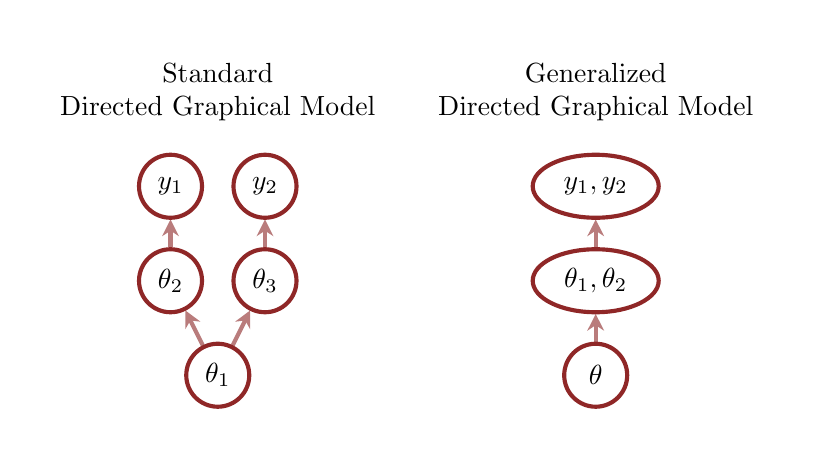
\begin{tikzpicture}[scale=0.2, thick]

  \pgfmathsetmacro{\r}{2}
    
  \begin{scope}[shift={(0, 0)}]
    \draw[white] (-12, -4) rectangle (12, 22);
  
    \node[align=center] at (0, 18) { Standard\\Directed Graphical Model };
  
    \coordinate (A) at (0, 0);
    
    \coordinate (B) at (-3, 6);
    \coordinate (C) at (+3, 6);
    
    \coordinate (D) at (-3, 12);
    \coordinate (E) at (+3, 12);

    \foreach \B/\E in {A/B, A/C, B/D, C/E} {
      \draw[-{Stealth[length=6pt, width=6pt]}, shorten <=12.1, shorten >=12, color=mid, line width=1.5] (\B) -- (\E);
    }

    \filldraw[fill=white, draw=dark, line width=1.5] (A) circle (\r)
    node[color=black] { $\theta_{1}$ };

    \filldraw[fill=white, draw=dark, line width=1.5] (B) circle (\r)
    node[color=black] { $\theta_{2}$ };
    
    \filldraw[fill=white, draw=dark, line width=1.5] (C) circle (\r)
    node[color=black] { $\theta_{3}$ };
    
    \filldraw[fill=white, draw=dark, line width=1.5] (D) circle (\r)
    node[color=black] { $y_{1}$ };
    
    \filldraw[fill=white, draw=dark, line width=1.5] (E) circle (\r)
    node[color=black] { $y_{2}$ };

  \end{scope}

  \begin{scope}[shift={(24, 0)}]
    \draw[white] (-12, -4) rectangle (12, 22);
  
    \node[align=center] at (0, 18) { Generalized\\Directed Graphical Model };
    
    \coordinate (A) at (0, 0);
    \coordinate (B) at (0, 6);
    \coordinate (C) at (0, 12);

    \draw[-{Stealth[length=6pt, width=6pt]}, shorten <=12.1, shorten >=12, color=mid, line width=1.5] (A) -- (B);
    \draw[-{Stealth[length=6pt, width=6pt]}, shorten <=12.1, shorten >=12, color=mid, line width=1.5] (B) -- (C);

    \filldraw[fill=white, draw=dark, line width=1.5] (A) circle (\r)
    node[color=black] { $\theta$ };

    \filldraw[fill=white, draw=dark, line width=1.5] (B) circle [x radius={2 * \r}, y radius={1 * \r}]
    node[color=black] { $\theta_{1}, \theta_{2}$ };
    
    \filldraw[fill=white, draw=dark, line width=1.5] (C) circle [x radius={2 * \r}, y radius={1 * \r}]
    node[color=black] { $y_{1}, y_{2}$ };

  \end{scope}

\end{tikzpicture}

\end{document}  